\input{../header}
\usepackage{pgfplots}
\rhead{Your name: \rule{8cm}{0.15mm}}

\begin{document}

\section{Learning target IN2 and INx, version 1}

\iffalse
IN2: Find approximations to definite integrals using variations of Riemann sums.

INx: Correctly interpret the meaning of an area under a curve using the ideas of net change, displacement, etc. Apply the appropriate units to the value.

\hrulefill
\fi

The rate at which pollution escapes a scrubbing process at a manufacturing plant increases over time as filters and other technologies become less effective. Suppose that the rate of pollution (measured in tons per week) is given by the function $r$ that is pictured below. Throughout this problem, we're interested in $\displaystyle\int_{t=0}^5 r(t)\, dt$.

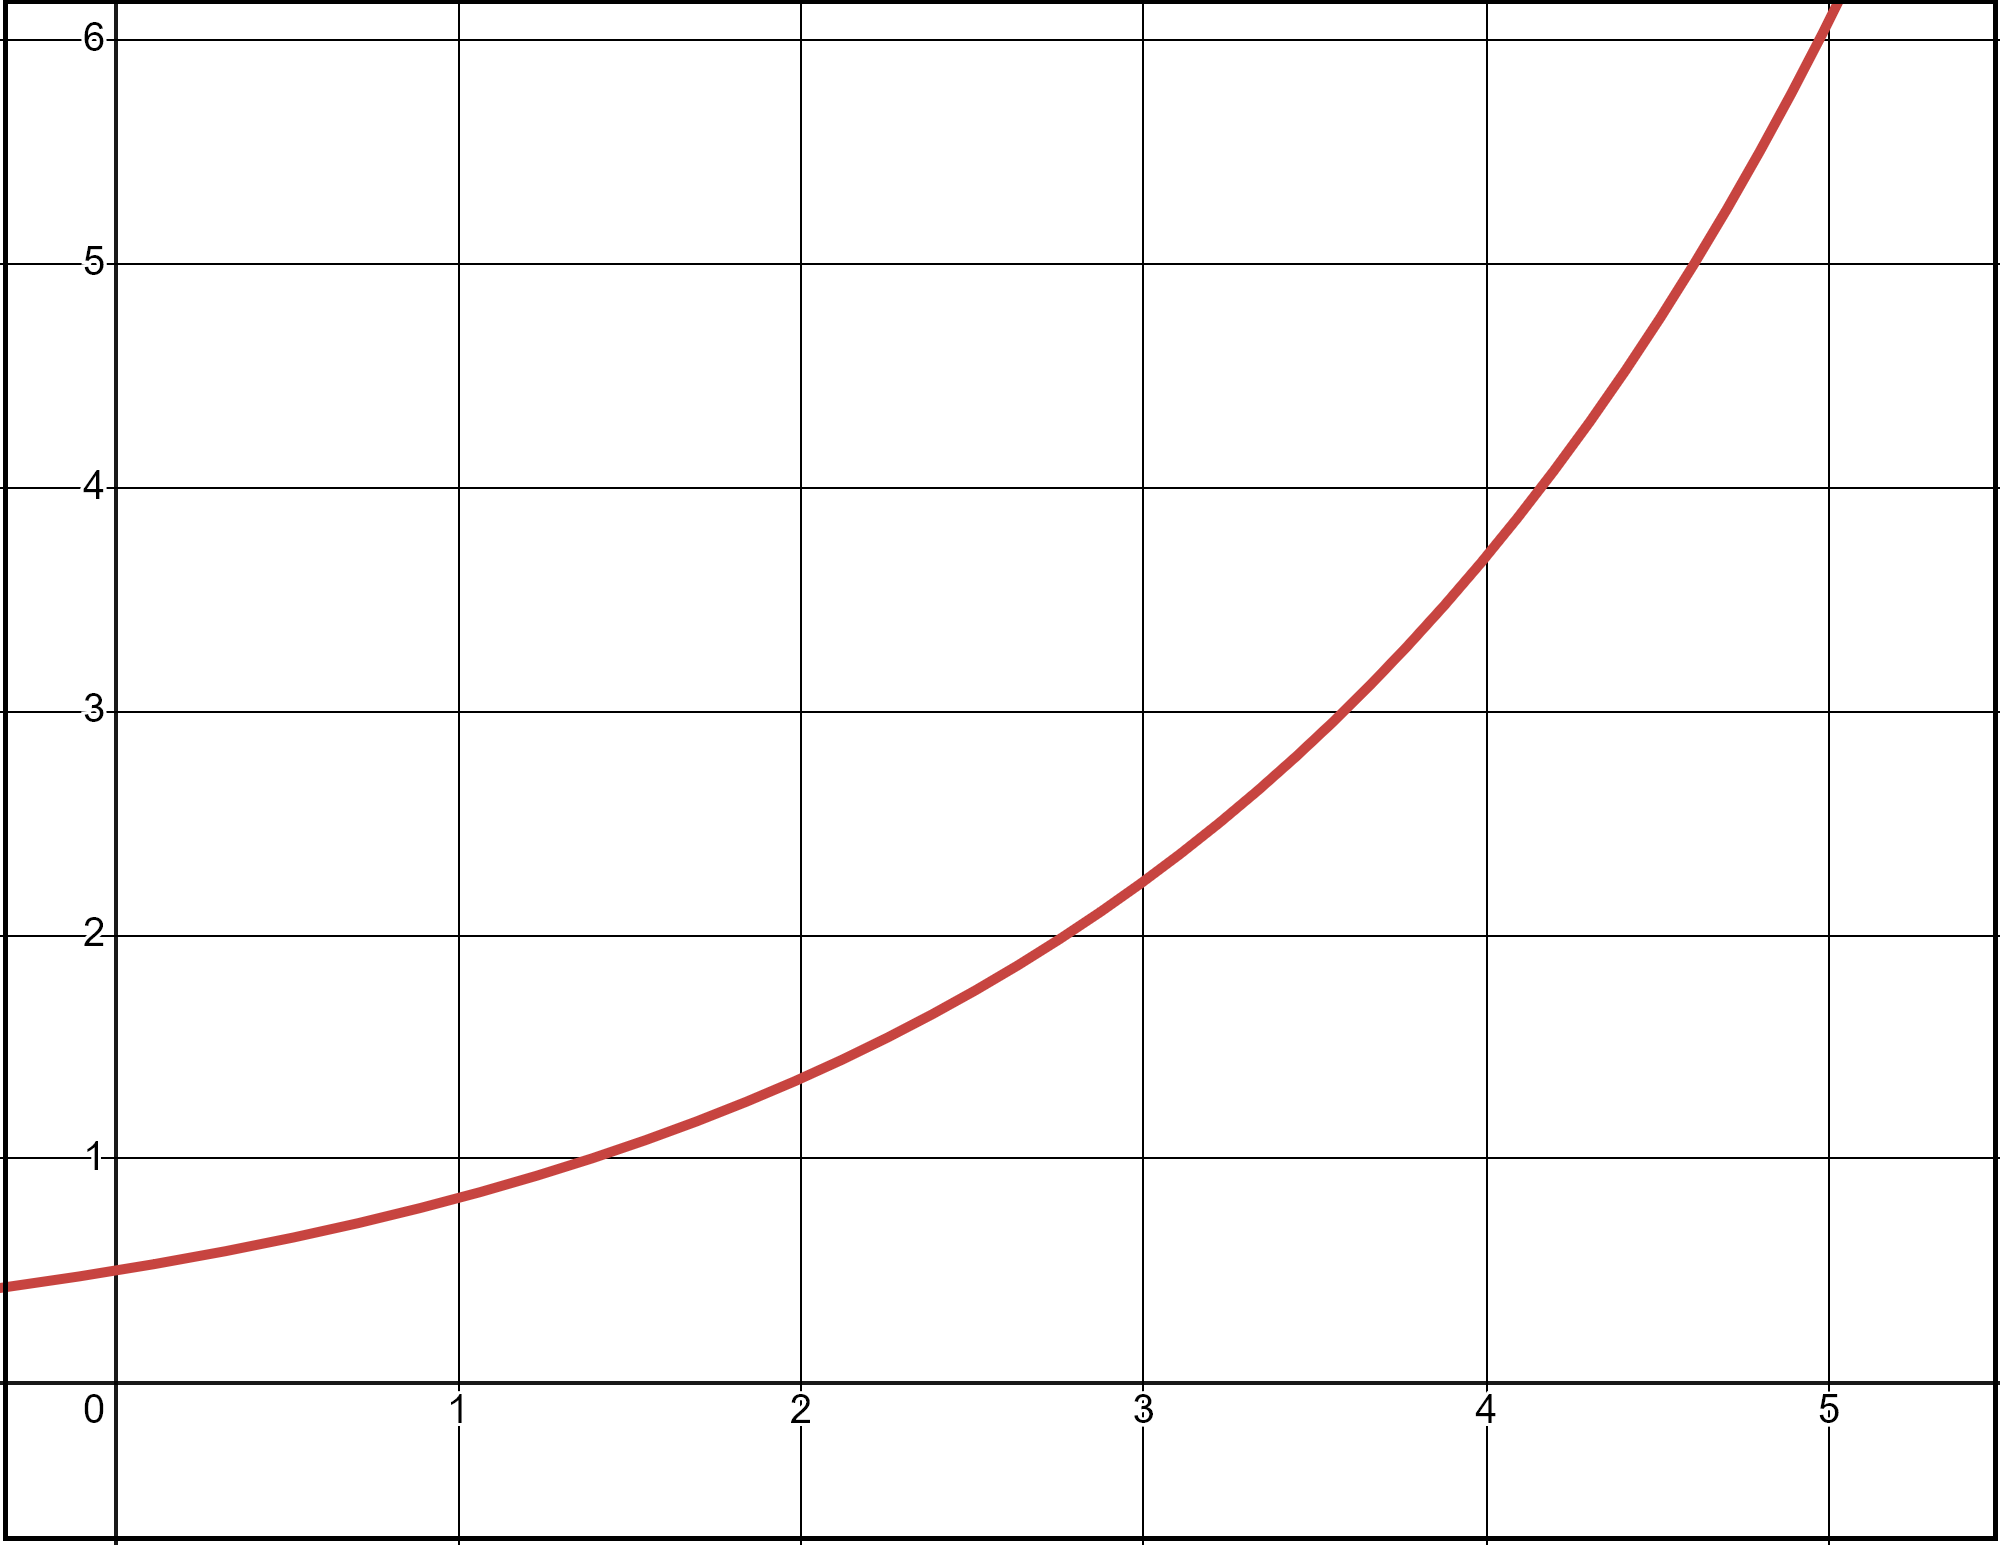
\includegraphics[width=0.5\textwidth]{../images/IN2-v1.png}
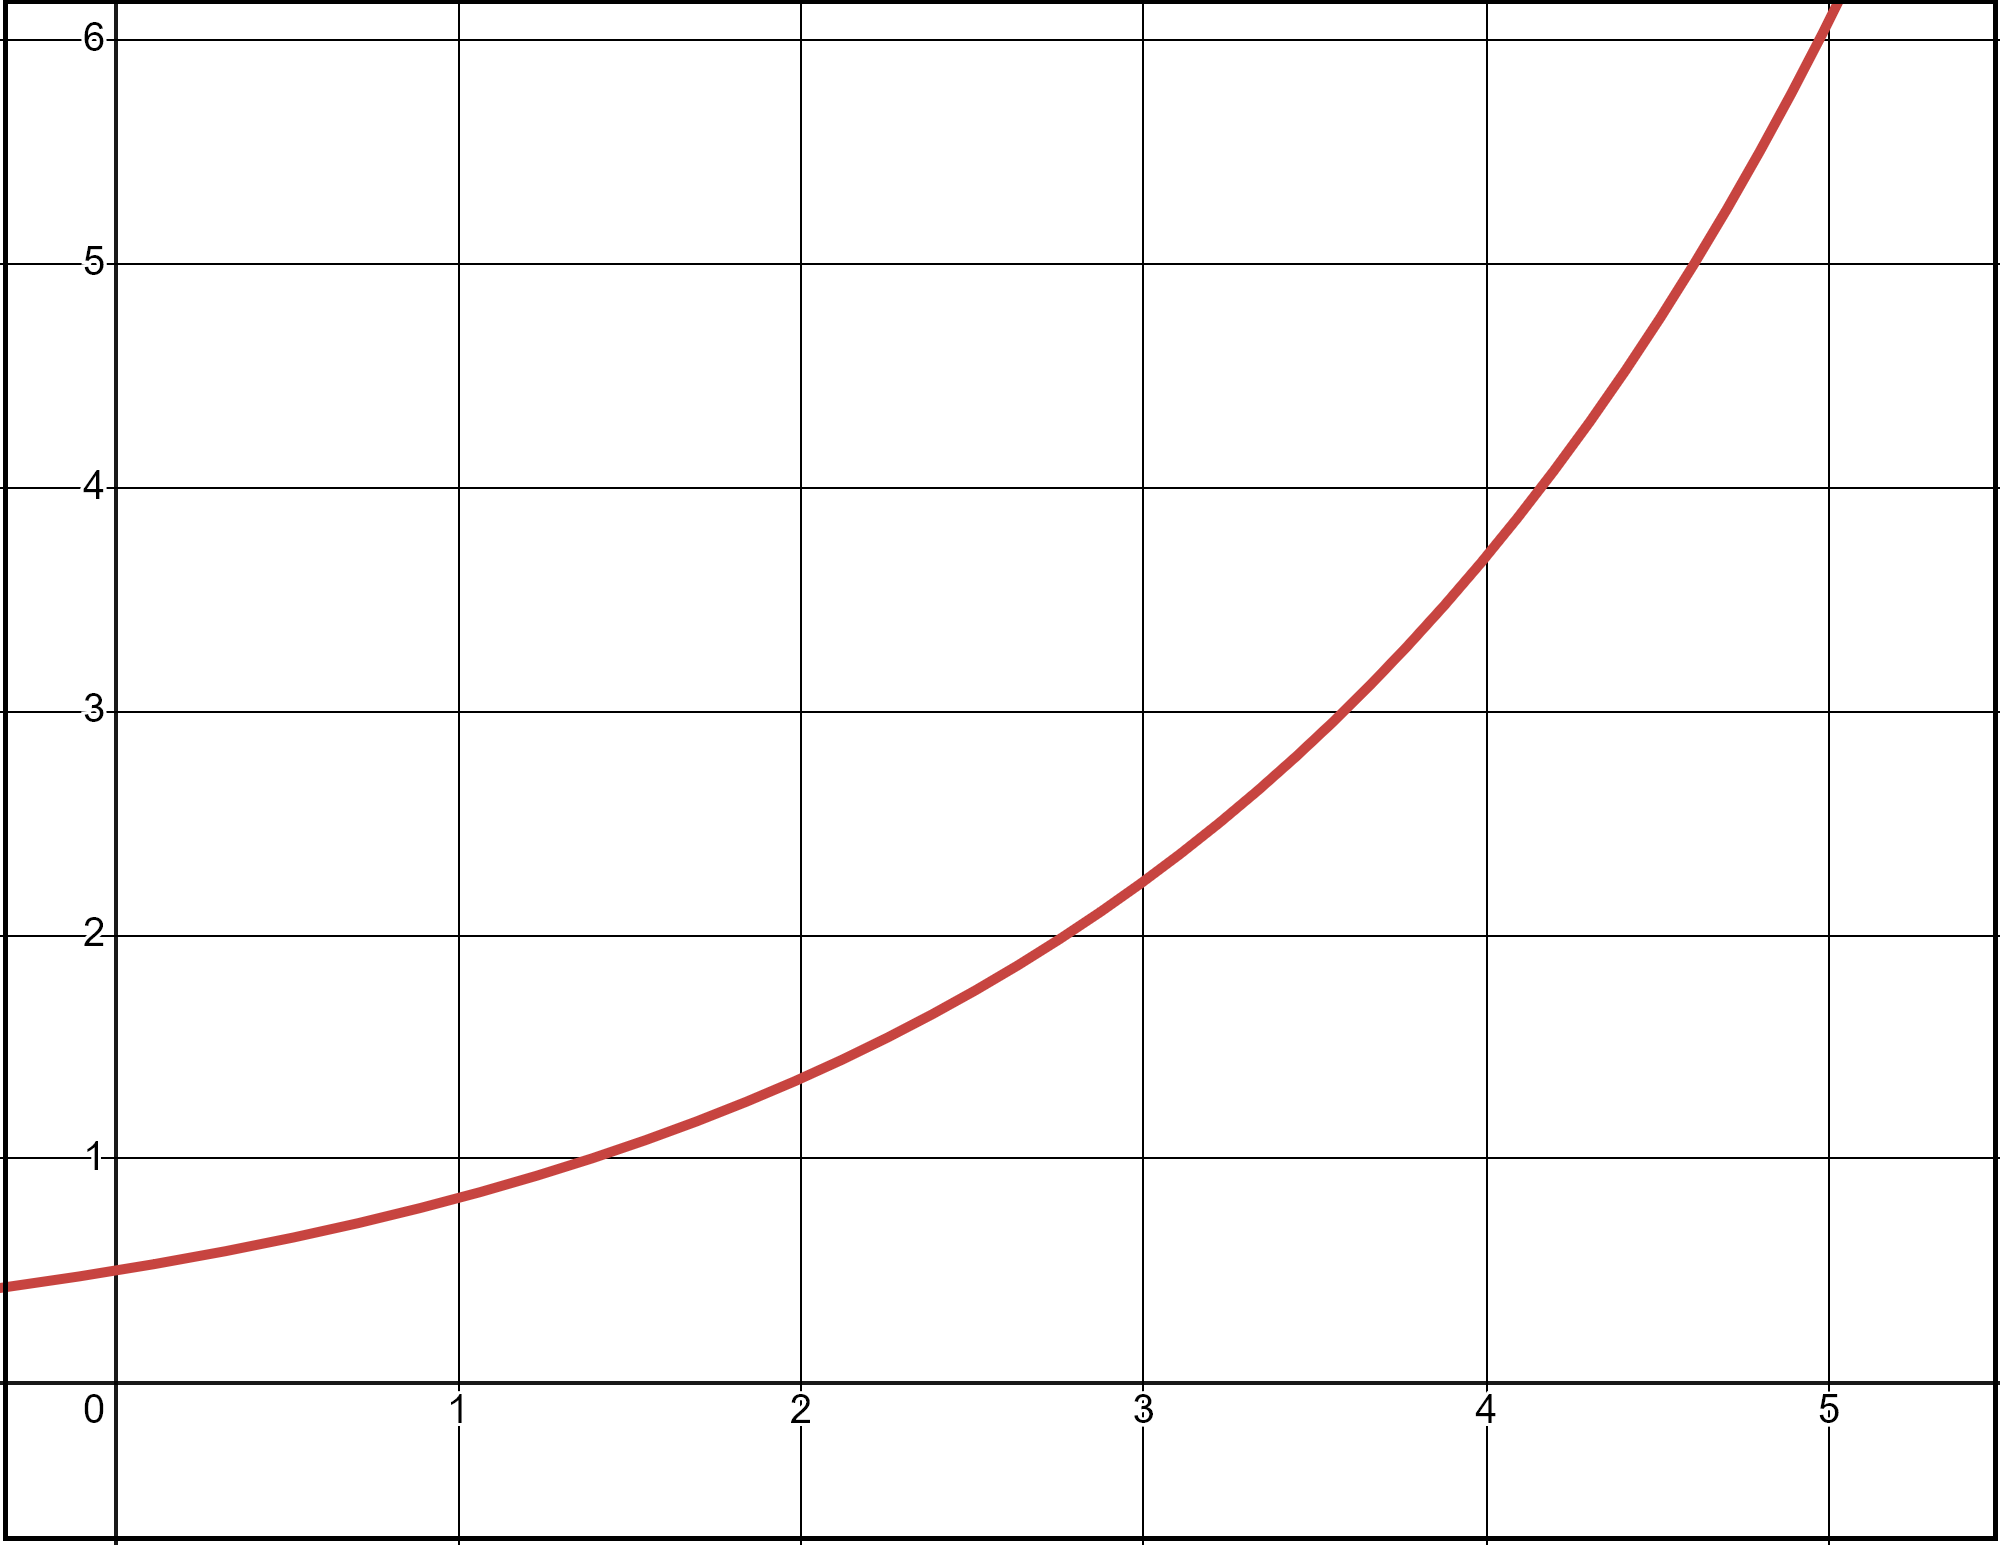
\includegraphics[width=0.5\textwidth]{../images/IN2-v1.png}
\begin{enumerate}[(a)]
\item On the first graph above, carefully draw the \textit{left} Riemann sum with four rectagles of uniform width. (How wide should each rectangle be?)
\item On the second graph above, carefully draw the \textit{right} Riemann sum with four rectangles.
\item If $r(t) = 0.5 e^{0.5t}$, compute both of these Riemann sums. Show your work for computing the heights of the rectangles. (Hint: lots of your work will overlap!)

\textbf{Include units on every number you write.}
\vfill
\item Give your best guess for $\displaystyle\int_{t=0}^5 r(t)\, dt$, \textbf{include units}, and explain what this number means about pollution.
\end{enumerate}
%%%%%%%%%%%%%%%%%%%%%%%%%%%%%%%%%%%%%%%%%%%%%%%%%%%%%%%%%
\pagebreak
%%%%%%%%%%%%%%%%%%%%%%%%%%%%%%%%%%%%%%%%%%%%%%%%%%%%%%%%%

\section{Learning target IN2 and INx, version 2}

\iffalse
IN2: Find approximations to definite integrals using variations of Riemann sums.

INx: Correctly interpret the meaning of an area under a curve using the ideas of net change, displacement, etc. Apply the appropriate units to the value.

\hrulefill
\fi

A colony of bacteria in a petri dish is growing at a rate of 
\(f(t) = 1.75^t\, \text{million bacteria per hour}\). Let's figure out how much the colony grows over the course of three hours.

\fbox{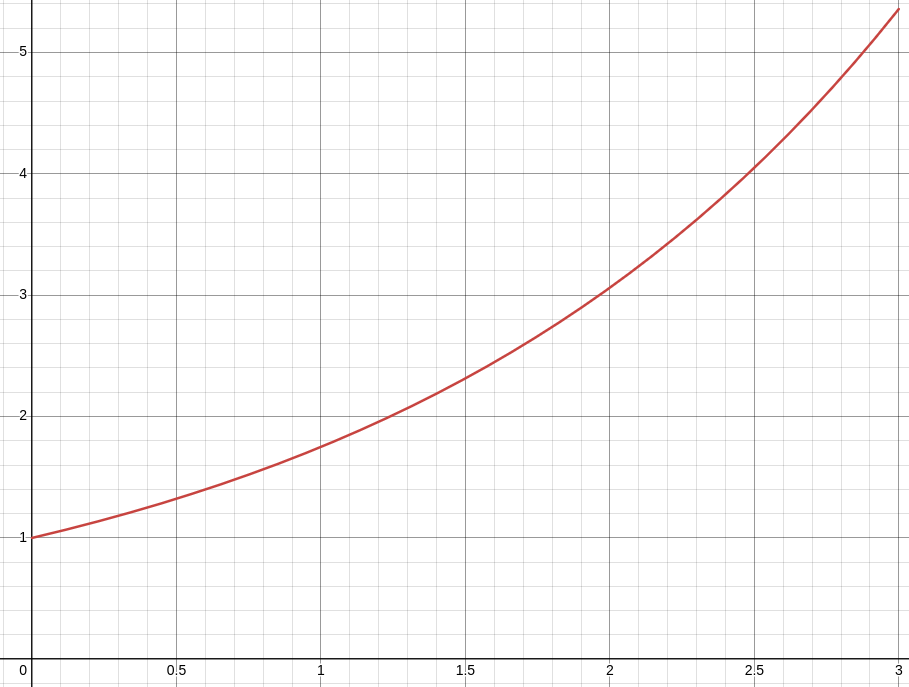
\includegraphics[width=0.5\textwidth]{../images/IN2-v2.png}}
\fbox{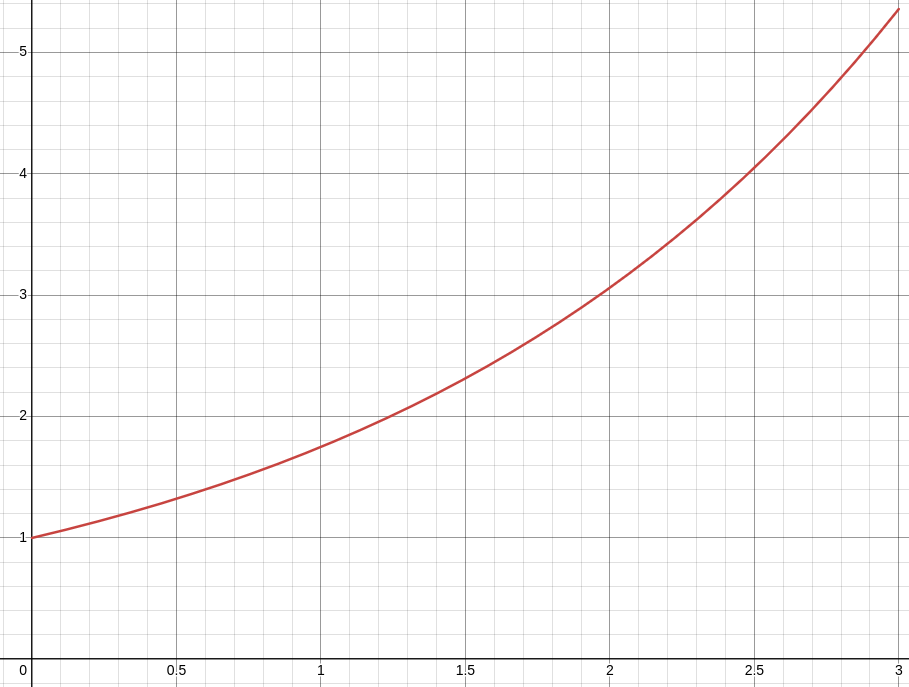
\includegraphics[width=0.5\textwidth]{../images/IN2-v2.png}}
\begin{enumerate}[(a)]
\item On the first graph above, carefully draw the \textit{left} Riemann sum with four rectagles of uniform width. (How wide should each rectangle be?)
\item On the second graph above, carefully draw the \textit{right} Riemann sum with four rectangles.
\item Compute both of these Riemann sums. Show your work for computing the heights of the rectangles. (Hint: lots of your work will overlap!)

\textbf{Include units on every number you write.}
\vfill
\item Give your best guess for $\displaystyle\int_{t=0}^3 f(t)\, dt$, \textbf{include units}, and explain what this number means about the bacteria colony.
\end{enumerate}
\end{document}